% % !TEX TS-program = pdflatex
% % !TEX root = ../tesi.tex
%
% %************************************************
% \chapter{Acustica}
% \label{chp:Acustica}
% %************************************************
%
% Questo capitolo affronta il processo della produzione, dispersione e percezione dell'onda sonora. Il campo della scienza che si occupa degli studi relativi alla fisica del suono si chiama \emph{acustica}, i cui primi passi sono stati mossi già dai primi \textit{pitagorici} portando innovazione ancora oggi. Di studi più recenti sulla percezione dell'evento sonoro da parte dell'uomo se ne occupa invece la \textit{psicoacustica}.
%
% \section{Il Suono}
%
% Per sintetizzare un riverberatore è necessario prima comprendere, dal punto di vista fisico, cosa accade nel momento in cui un suono viene generato e del suo comportamento nello spazio circostante.
%
% Per \textbf{\textit{suono}} intendiamo un'alterazione di pressione, velocità e posizione delle particelle, propagata in un mezzo elastico, o la sovrapposizione di tali alterazioni.
% Parlando di suono ci riferiamo anche alla percezione definita dal nostro sistema uditivo delle alterazioni sopracitate (H. F. Olson - Elements of acoustical engineering - 1957 pag2).
%
% Il suono è prodotto quando il mezzo di propagazione (nella maggior parte dei casi l'aria)
% è messo in vibrazione da un qualsiasi evento di natura meccanica, per esempio, l'oscillazione di una corda o il battere di un oggetto su una superficie solida  (Harry f.olson - Elements of acoustical engineering - 1957 pag 2).
%
% Queste vibrazioni, propagate in modo sferico, raggiungono il nostro orecchio avente la funzione di trasduttore (trasforma l'energia cinetica in impulsi elettrici) risultando nella nostra percezione dell'evento sonoro.
%
% \subsection{Caratteristiche}
% Le caratteristiche principali, sempre dal punto di vista fisico del suono percepito sono dunque:
% \begin{itemize}
%       \item \emph{Periodo}:
%       Il tempo di completamento di un ciclo (ovvero quando, un segnale periodico esprime tutti i suoi valori ricorrenti) espresso in secondi
%       \item \emph{Frequenza}:
%       il numero di cicli in 1 secondo, si esprime in hertz
%       \item \emph{Lunghezza d'onda}:
%       la distanza tra 2 massimi consecutivi, si esprime in metri
%       \item \emph{Ampiezza}:
%       massima escursione dal punto di equilibrio
%       \item \emph{Velocità dell'onda}:
%       velocità di movimento del fronte d'onda nel mezzo, si esprime in metri al secondo.
% \end{itemize}
% (D. Davis - Sound System Engineering - 2013 pag 171)
% \bigskip
%
% Ovviamente queste caratteristiche non sono universali ma dipendono da fattori ambientali che ne definiscono i valori. Due eventi sonori, di partenza identici, non verranno percepiti ugualmente al variare delle condizioni esterne.
% Queste condizioni che influiscono sul suono sono:

\section{Acustici Luoghi Comuni}

\todo[inline]{in questa sezione\ldots bla bla bla}

\subsection{Distanza dalla sorgente}

La distanza dalla sorgente sonora è risaputo comportare una diminuzione di
intensità. Dato che l’onda si propaga in modo sferico, segue la legge
dell’inverso del quadrato, comportando una diminuzione di 6 db ad ogni raddoppio
della distanza.

\subsection{Conformazione del gas/Temperatura e densità}

Parlare di temperatura è importante in quanto è un fattore che influisce in
diversi altri fattori presi in esame in questa tesi, ed è inoltre il punto di
partenza della mia ricerca.
Dalla temperatura dipendono infatti la velocità del suono nel mezzo e il valore
di assorbimento atmosferico.
La velocità del suono possiamo calcolarla secondo la seguente formula:

\begin{equation}
C=\sqrt{\frac{\gamma Ps}{\rho}}
\end{equation}
dove

\begin{itemize}
      \item $\gamma$ è il coefficiente di dilatazione adiabatica
      \item $Ps$ è la pressione circostante
      \item $\rho$ è la densità del gas
\end{itemize}

La densità del gas, come per il coefficiente di dilatazione adiabatica, varia a
seconda della temperatura che, data la sua presenza in varie equazioni, diviene
un fattore determinante per la velocità del suono e dunque per le
caratteristiche del riverbero.
Possiamo calcolare la densità tramite la seguente formula (pag 173):
\begin{equation}
\rho = \frac{stp*hg}{1+(t*hg*0.00367)}
\end{equation}

di cui:

\begin{itemize}
      \item $stp$ è la densità del gas a temperatura e pressione standard;
      \item $hg$ è la pressione barometrica del mercurio in centimetri;
      \item $t$ è la temperatura in gradi Celsius;
      \item $0.00367$ è il  coefficiente di dilatazione termica,una costante comune a tutti i gas
\end{itemize}

Possiamo verificare la densità standard dei gas a tabella \ref{tab:dens}

\bigskip
\begin{table}[h]
\centering
\caption{Tabella raffigurante la densità di alcuni gas a \emph{}}
\label{tab:dens}
\begin{tabular}{lcr}
\toprule
Nome del gas & Simbolo & Densità($kg/m^2$) \\
\midrule
Aria & - & 1.2930 \\
Ammonia & $NH_3$ & 0.7710 \\
Nitrogen & $N_2$ & 1.2507 \\
Chlorine & $CI_2$ & 3.2170 \\
Carbon dioxide & $CO_2$ & 1.9760 \\
Hydrogen & $H_2$ & 0.0899 \\
Methane & $CH_4$ & 0.7170 \\
Carbon Monoxide & $CO$ & 1.2500 \\
Oxygen & $O$ &1.4290 \\
Water Vapour & $H_2O$ & 0.804 \\
\bottomrule
\end{tabular}
\end{table}
\smallskip

\subsubsection{Assorbimento atmosferico}
Rappresenta l’effetto di dissipazione dell’energia data dall’azione combinata
di viscosità e calore del mezzo. Perdite di energia aggiuntive sono dovute
all’umidità assoluta. Questo effetto comporta inoltre un aumento
dell’attenuazione con l’aumento delle frequenze.
\begin{figure}[h]
\centering
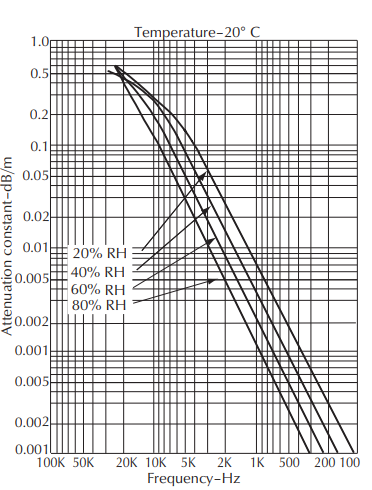
\includegraphics[width=%
0.50\textwidth]{assorbimento}
\caption{Tabella dei coefficenti di assorbimento dell'aria}
\label{fig:assorbimento}
\end{figure}

\subsubsection{Umidità}
Il livello di umidità del gas si riferisce alla presenza o meno di molecole
d’acqua nel mezzo. La sua influenza non è tanto impattante per quanto riguarda
la velocità dell’onda, ma sull’assorbimento acustico totale comportando un
abbattimento di intensità a diverse frequenze.

\subsubsection{Fenomeni di Riflessione}

Le riflessioni sono alla base di ciò che chiamiamo riverbero.
Consistono nella riflessione di un’onda sonora sulle diverse superfici che
circondano l’evento acustico, esse siano pareti oppure oggetti che si interpongono
nella propagazione dell’onda.

Affinché ci sia una riflessione, la superficie riflettente deve necessariamente
essere
più larga di almeno $\frac{1}{4}$ della lunghezza d’onda.
Quando l’oggetto è più piccolo di questa soglia si ha una diffrazione, ovvero
l’onda sonora curva attorno ad esso.

Un altro fenomeno, che possiamo considerare inverso alla riflessione, è \emph{l’assorbimento}.
L’assorbimento è dovuto alle proprietà del materiale che, appunto, al posto di riflettere l’onda assorbono parte dell’energia, trattenendola e restituendo un’onda smorzata.
Più un materiale è assorbente, più sarà rapido il decadimento dell’energia sonora nello spazio fino a tornare in una situazione di stabilità.
La condizione di stabilità sussiste infatti, quando la quantità di energia assorbita è la medesima dell’energia prodotta.

\subsubsection{Fenomeni di Rifrazione}

La rifrazione similmente alla riflessione si ha quando è il mezzo di trasmissione a subire delle variazioni, comportando dunque una differenza nella propagazione in atto. Queste variazioni possono essere, per esempio, temperatura, densità o direttamente un mezzo diverso, basti pensare ad un onda prodotta in aria che incontra una superficie d’acqua.

\section{Psicoacustica}

Altro aspetto da tenere in considerazione è il nostro sistema uditivo. In un sistema lineare in frequenza data in input una lista di frequenze, l’output conterrà le stesse, anche se magari dissimili in ampiezza e fase.
Il nostro apparato uditivo, infatti, a causa di secoli di evoluzione e cambiamenti ha sviluppato dei comportamenti che non lo rendono un sistema lineare, portando dunque a delle inesattezze dal punto di vista percettivo.
Ecco alcuni esempi di fenomeni di non linearità a cui siamo sottoposti:

\begin{itemize}
\item Distorsione armonica:
È la percezione di armoniche superiori di un tono puro. Questa distorsione può essere dovuta ad una pressione eccessiva dell’onda sul timpano;
\item Tono di combinazione:
Detto anche \textit{“terzo suono di Tartini”} è un effetto psicoacustico che comporta nella percezione di un terzo suono, nonostante in input i suoni siano stati solo 2.
La frequenza del tono ricostruito non sarebbe altro che la differenza tra i 2 toni di partenza
\item Curve isofoniche:
Il fenomeno delle curve isofoniche comporta una diversa percezione di ampiezza a per diverse frequenze ma aventi stesso SPL. Per fare un esempio una sinusoide da 1000 Hz a 110 Db SPL ha la stessa percezione di una sinusoide da 3000 Hz ma a 100 Db SPL (ballou - Handbook for Sound Engineers - 2008 - pag 43).
\end{itemize}

\begin{figure}[h]
\centering
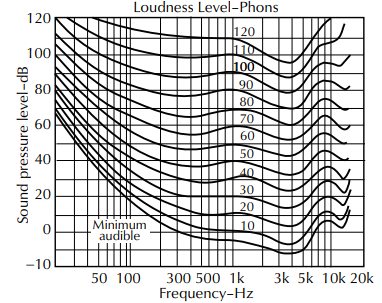
\includegraphics[width=%
0.50\textwidth]{isofoniche}
\caption{Grafico che mostra il comportamento delle curve isofoniche}
\label{fig:isofoniche}
\end{figure}
Questo è anche il motivo per il quale siamo più sensibili nella banda intorno ai 4 KHz, comportando dolore nell’ascoltatore se sottoposto a db elevati.
\subsubsection{Percezione della distanza}
Più interessante ai fini della tesi è la percezione della distanza, tema chiave nello studio degli spazi e della propagazione del suono.
È noto che, duplicata la distanza tra fonte sonora e ascoltatore, il SPL decade di 6 dB.
Nonostante questo, affinché abbiamo la percezione della duplicazione della distanza c’è bisogno della diminuzione di almeno 20 dB (j. Blauert spatial hearing).

Un elemento che però ci permette di comprendere quando una fonte è lontana è la sua composizione spettrale, infatti, a causa dell’assorbimento dell’aria (del mezzo per essere più precisi) le frequenze alte saranno assorbite maggiormente, comportando una presenza più elevata di basse frequenze.

Per questo, in modo tale da replicare distanza e vicinanza dalla fonte sonora, oltre a questi accorgimenti è da tenere in considerazione il rapporto tra suono diretto e riverberato.
In un ambiente reale infatti, è proprio il rapporto tra le due sorgenti a determinare dove e quanto è distante un evento sonoro.

\section{Spazio}
Come citato poc'anzi quando si parla di suono bisogna considerare quindi lo spazio e il mezzo in cui l'onda si propaga.
Possiamo classificare gli spazi in diverse categorie, le principali sono (Davis - Pag 178):
\begin{itemize}
\item Free Field:
È definito così uno spazio uniforme, libero da ostacoli che potrebbero produrre delle riflessioni o rifrazioni e non contaminato da sorgenti sonore estranee.
Esempi di questo tipo sono le sale anecoiche (senza eco),camere particolari il cui scopo è quello di ridurre al minimo le riflessioni delle onde, utili per eseguire test precisi su apparecchiature audio.
\item Reverberant field:
È uno spazio chiuso, con pochissimo assorbimento acustico, in cui la pressione sonora è uniforme in ogni punto e le onde si propagano allo stesso modo in tutte le direzioni.
Caratteristiche di questo tipo possiamo trovarle in luoghi come camere vuote o cavità.
\item Semireverberant Field:
È il tipo di spazio più comune che possiamo incontrare, nel quale l’energia è sia assorbita che riflessa. L’energia si muove in più direzioni ma è comunque percepibile il punto di origine della fonte di generazione dell’evento sonoro.
\end{itemize}
\subsection{Risposta all'impulso}
Al giorno d’oggi conosciamo una tecnica in grado di eseguire una fotografia delle caratteristiche acustiche in grado di descrivere come il suono si propaga da un punto di emissione ad un ricevitore.

Parliamo di \textit{Risposta all’impulso} ovvero del modello fisico-matematico di un sistema lineare, non dipendente dal tempo, composto solo da un input ed un output (A.Farina - ROOM IMPULSE RESPONSES AS TEMPORAL AND SPATIAL FILTERS - 2006).

Le informazioni contenute sono sia relative al dominio del tempo, ad esempio riflessioni e ritardi nella propagazione che, relative al dominio della frequenza, comportando quindi modifiche dal punto di vista spettrale.

Il sistema utilizzato viene detto \textit{Black box} che, come detto in precedenza è composto da un singolo input ed un singolo output. All’interno di questa black box gli elementi che concorrono all’acquisizione dei dati matematici dello spazio che si vuole registrare sono:
\begin{itemize}
\item Un generatore di segnale: Tipicamente un pc;
\item Un amplificatore di segnale;
\item Un diffusore di segnale: il quale riproduce il segnale nello spazio in modo omnidirezionale;
\item Un ricevitore: un microfono anch’esso omnidirezionale, in quanto vogliamo escludere la direzionalità dallo studio.
\end{itemize}
Per misurare quindi la risposta all'impulso riproduciamo il segnale attraverso l’altoparlante nello spazio e contemporaneamente registriamo come, quel segnale, si propaga in quel determinato spazio e in quelle determinate condizioni, attraverso il microfono.

Il segnale originale consiste in uno sweep esponenziale il quale parte dalla frequenza $f_1$, termina a frequenza $f_2$ in $t$ secondi.

Il segnale riverberato conterrà al suo interno componenti spettrale non presenti nell’originale, che corrispondono alla risposta lineare in frequenza dello spazio.
Attraverso un processo di convoluzione, ampiamente spiegato e perfezionato dal prof. A Farina, siamo in grado di restituire la risposta all'impulso del sistema lineare.

È da tenere conto che però una singola registrazione non è in grado di descrivere tutto lo spazio. La risposta all’impulso, come già detto, è relativa soltanto al punto in cui è posizionato il ricevitore e soltanto per il punto da cui è emesso il suono. Per la mappatura dello spazio per restituire un'immagine fedele dello spazio sono necessarie numerose registrazioni. Come per una fotografia, maggiore è il numero di “pixel”, più definita sarà l’immagine. Per questo è un lavoro che, soprattutto per luoghi ampi, richiede moltissimo tempo e spesso si tende ad effettuare un numero di registrazioni non necessario a restituire un modello fedele.
\subsection{Storia dello studio degli spazi}
Storicamente, in ambito musicale, lo spazio è stato sempre presente ed essenziale durante le performance. Basti pensare agli auditorium greci, dove la conformazione permette sia un rinforzo in termini di ampiezza, ma anche una forte intelligibilità delle parole in modo tale da raggiungere chiaramente tutti i presenti.
Gli ascoltatori, posti ad un'angolazione di circa 120 gradi, ricevevano il suono diretto dall’oratore, seguito delle riflessioni provenienti sia dal pavimento dell’orchestra, che dal retro del palco, anche se con minor intensità.
\begin{figure}[h]
\centering
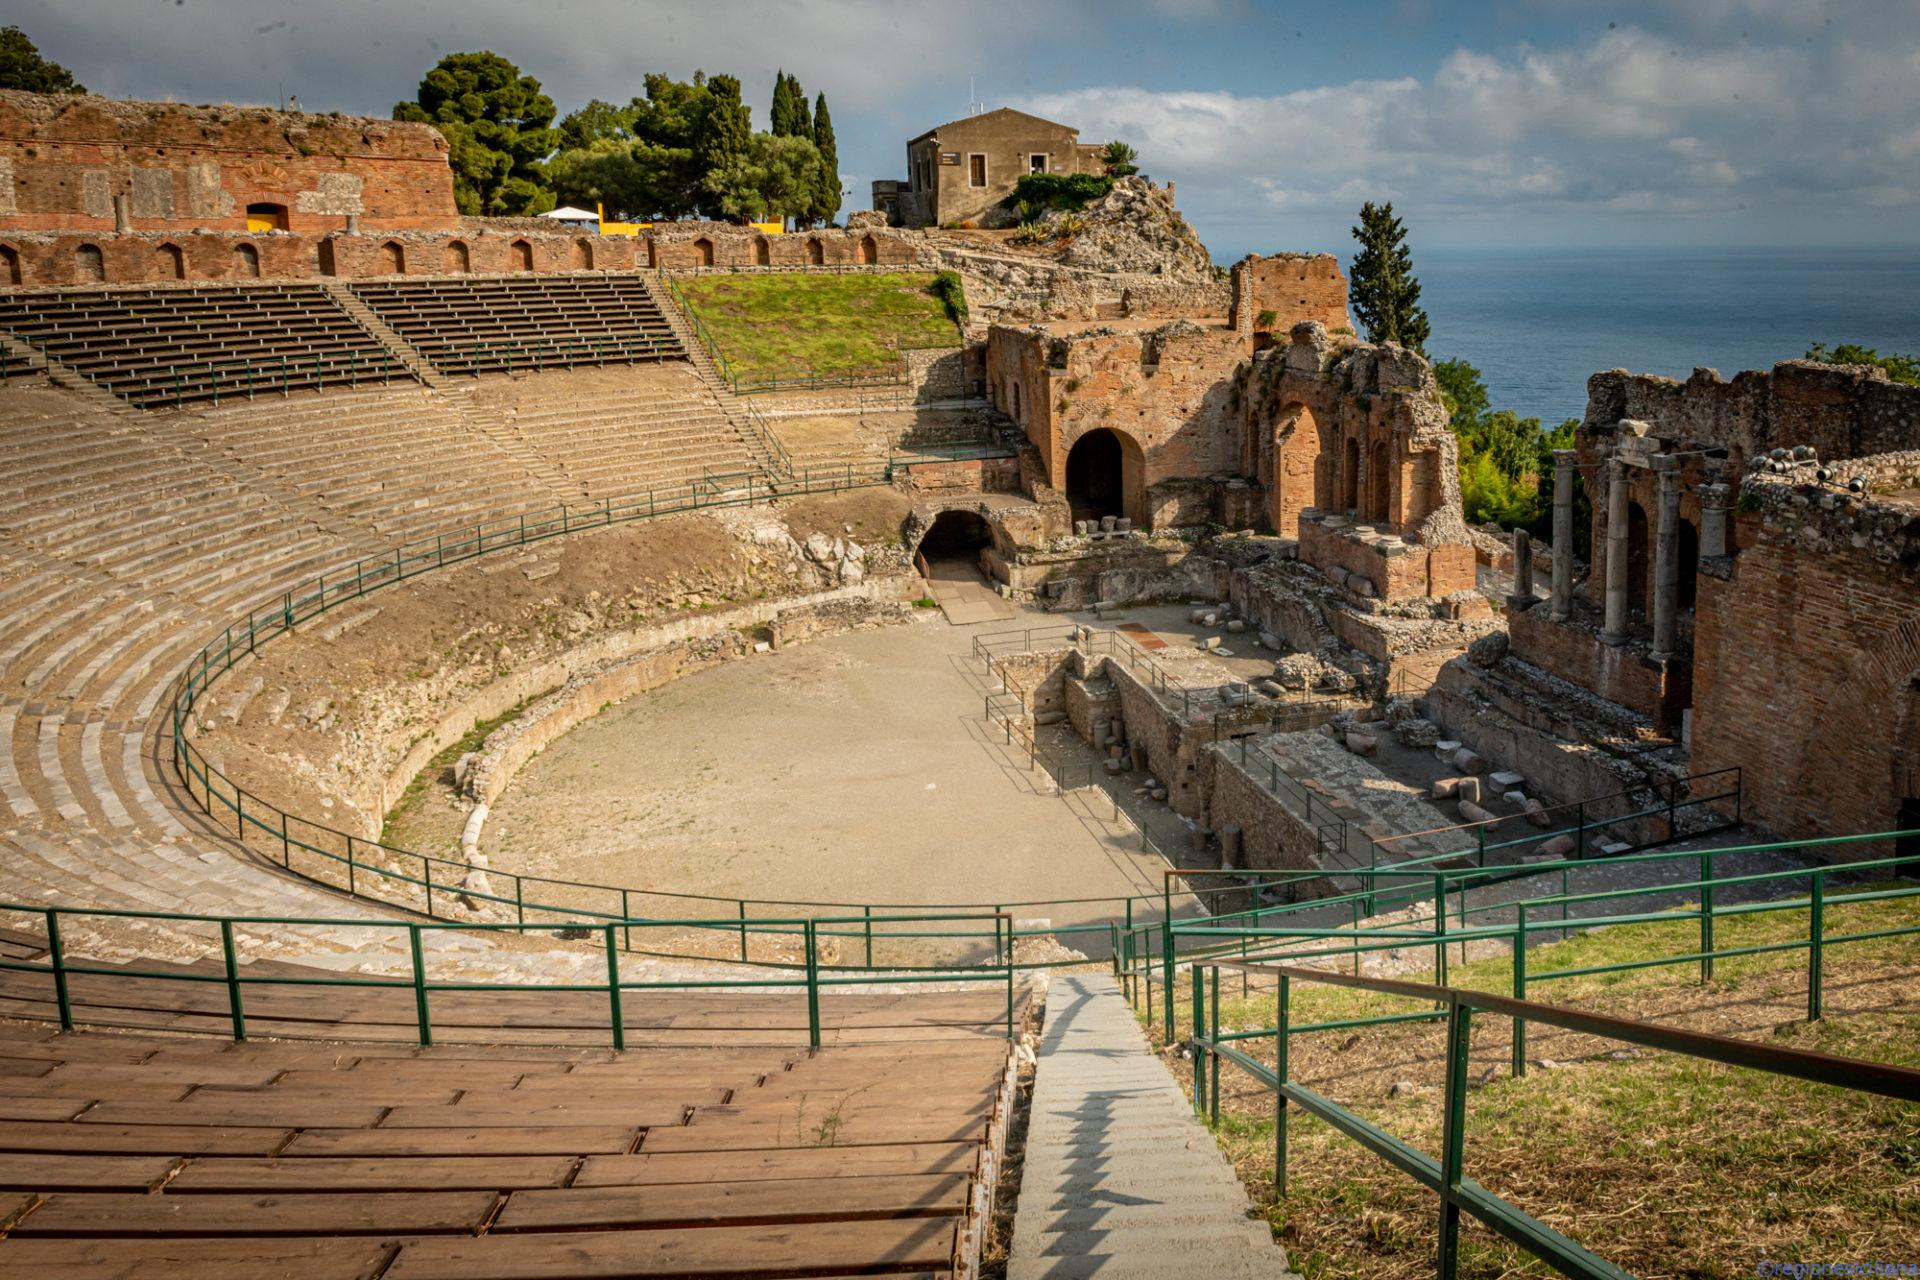
\includegraphics[width=%
0.50\textwidth]{teatrogreco}
\caption{Foto del teatro greco di Siracusa}
\label{fig:teatrogreco}
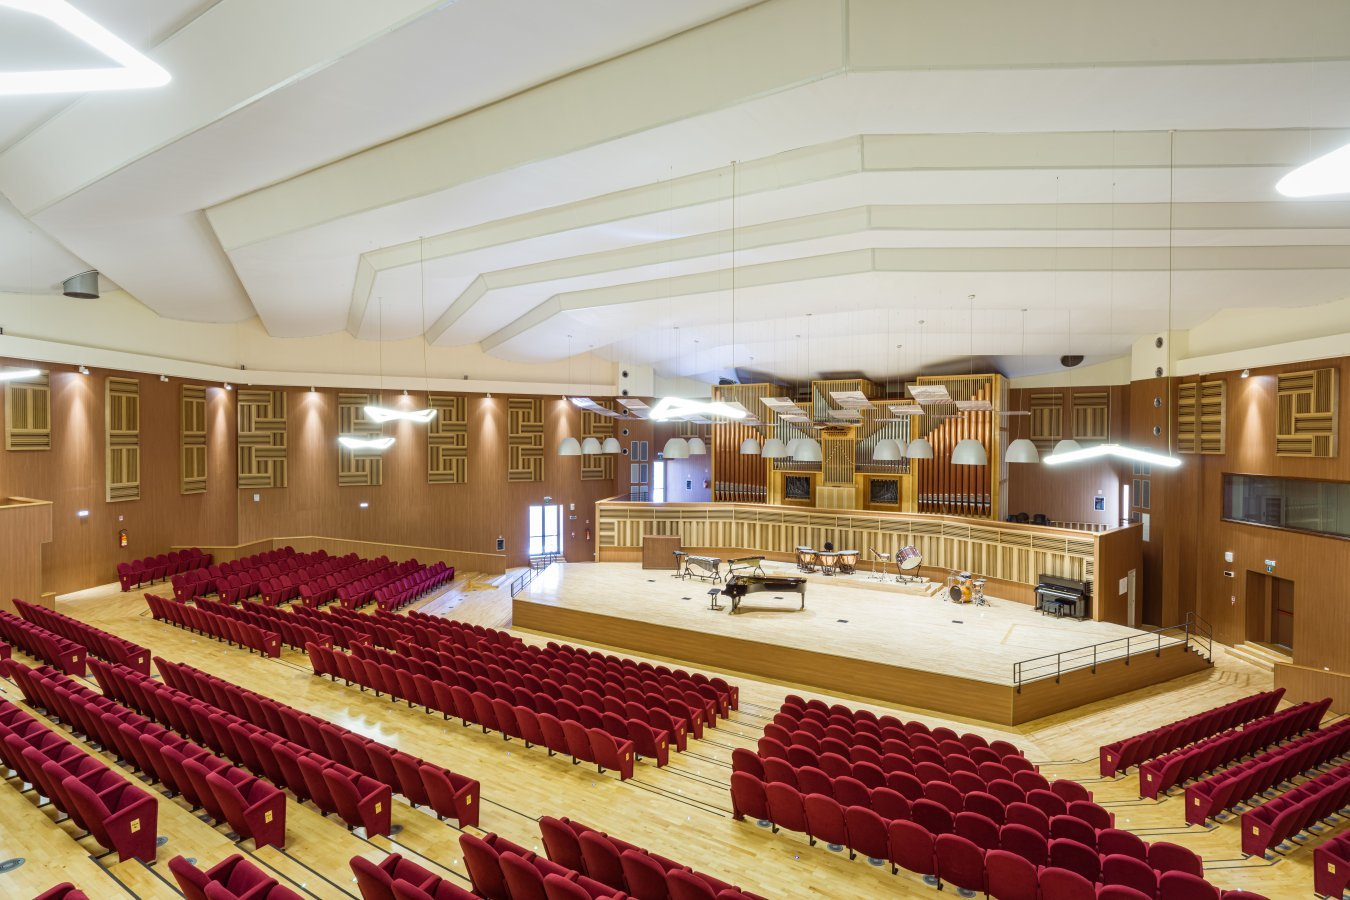
\includegraphics[width=%
0.50\textwidth]{auditorium}
\caption{Foto dell'auditorium Nino Rota del conservatorio di Bari}
\label{fig:auditorium}
\end{figure}
Il palco, inoltre, aveva un’ altezza compresa tra 1m e 3.6m, comportando una differenza nell’angolo di incidenza del suono diretto (Auditorium Acoustics and Architectural Design Di Michael Barron).
Infine, un altro accorgimento degli architetti greci, i quali avevano scoperto le proprietà di assorbimento, era il posizionamento tra le sedute di vasi contenenti ceneri, i quali avevano lo scopo di assorbire l’energia sonora che sarebbe stata riflessa indietro verso il palco.
\bigskip
Un’altro esempio in cui vediamo lo spazio come protagonista, è il caso degli organi, in cui il luogo è la vera e propria cassa armonica dello strumento.
L’acustica dell’organo è fortemente legata alla sua ubicazione, infatti, a differenza di altri strumenti musicali i quali possono essere spostati e trasportati, per l’organo non è possibile. Inoltre i luoghi provvisti di organo sono spesso molto riverberanti, come ad esempio le chiese e i teatri, e questo concorre alla definizione timbrica dello strumento
\begin{figure}[h]
\centering
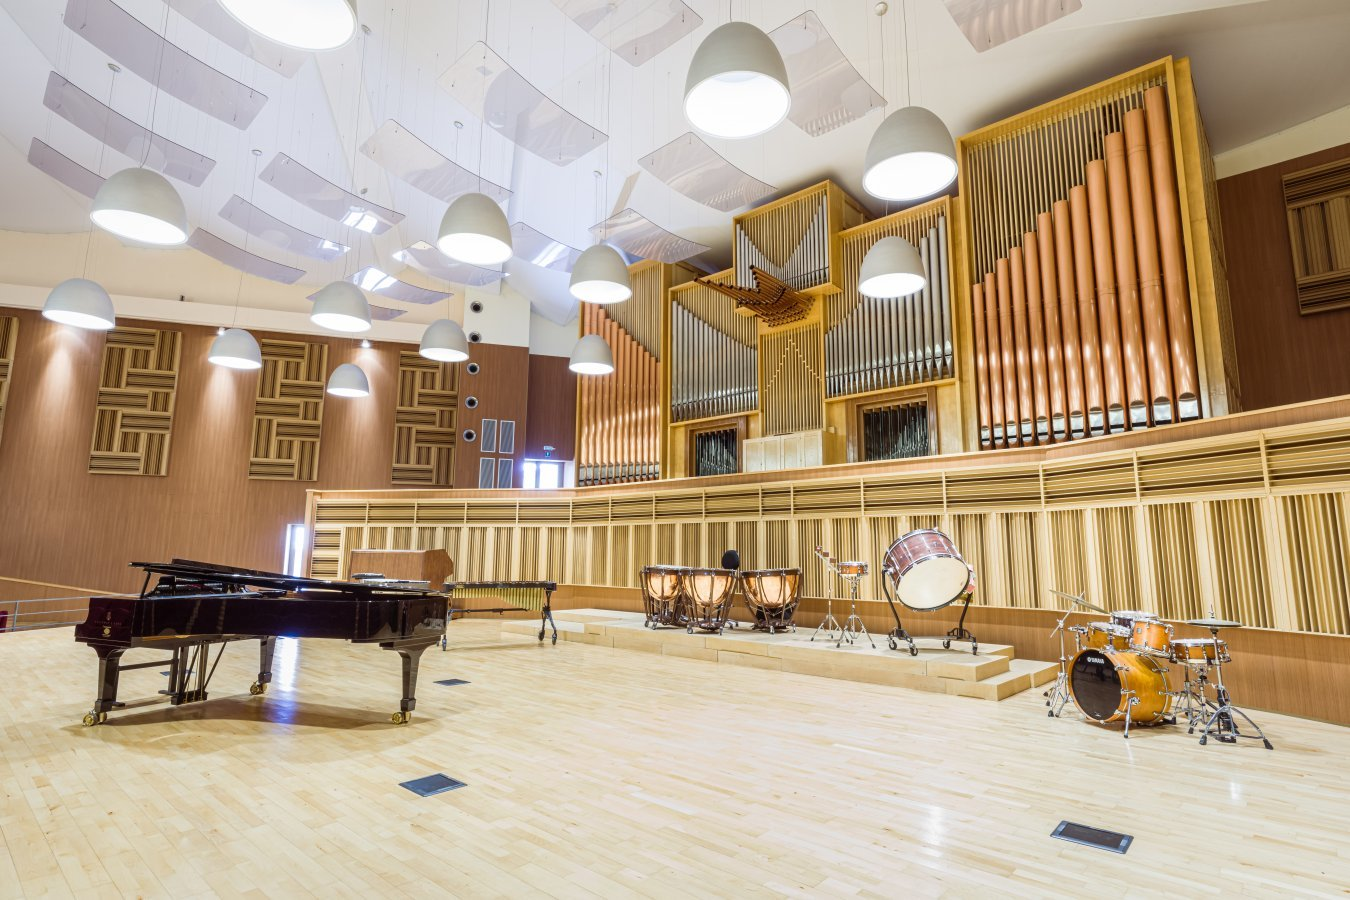
\includegraphics[width=%
0.50\textwidth]{organo}
\caption{Foto dell'organo presente nell'auditorium N.Rota}
\label{fig:organo}
\end{figure}
\subsubsection{Lo spazio come parametro}
Si è dovuto attendere però circa gli anni 60 affinchè lo spazio diventasse un vero e proprio parametro compositivo.

\emph{“Gesang der Jünglinge"} di Karlheinz Stockhausen è un’opera importantissima per l’epoca in cui è stata composta. Il brano, nato pentafonico e successivamente ridimensionato in quadrifonia, rappresenta l’avanguardia del serialismo integrale. Come accennato in precedenza, questo lavoro è il primo esempio in cui vediamo la gestione dello spazio come parametro compositivo, al pari di ampiezza, altezza e timbro.
Gli altoparlanti, disposti circolarmente attorno agli ascoltatori, creano uno spazio in cui immergersi permettendo complessi movimenti tra gli stessi.
Vengono infine introdotti termini quali “Intervallo spaziale” e “Accordi di spazio”.
